% % % % % % % % % % % % % % % % % % % % % % % % % % % % % % % % % % % % % % % %
% IEEE Style - Double columns, 11pt font, letterpaper
\documentclass[journal, twocolumn, final,11pt,letterpaper]{IEEEtran}	

% Include Latex Packages
\usepackage{etex}	% This package enables the use of many packages

% % Page styles
\usepackage{setspace}	% line spacing package
\doublespacing			% use double spacing
%\linespread{1.6}		% Use linespread to fine tune line spacing, not recommended


% % Figures
\usepackage{float}		% improves interface for floating objects
\usepackage{subfig}		% enables subfloat
\usepackage{graphicx}	% more image type support
\usepackage{circuitikz}
\usepackage{epstopdf}	% automatically convert included eps files to pdf
\usepackage{tikz}
%\usepackage{listings}
\usepackage{color}
\definecolor{dkgreen}{rgb}{0,0.6,0}
\definecolor{gray}{rgb}{0.5,0.5,0.5}
\definecolor{mauve}{rgb}{0.58,0,0.82}

\lstset{frame=tb,
	language=Verilog,
	aboveskip=3mm,
	belowskip=3mm,
	showstringspaces=false,
	columns=flexible,
	basicstyle={\small\ttfamily},
	numbers=none,
	numberstyle=\tiny\color{gray},
	keywordstyle=\color{blue},
	commentstyle=\color{dkgreen},
	stringstyle=\color{mauve},
	breaklines=true,
	breakatwhitespace=true,
	tabsize=3
}
\usetikzlibrary{matrix,calc}
\usetikzlibrary{shapes}

\newcommand*{\circled}[2][red]{
	\tikz[baseline=(char.base)]{
		\node[shape=ellipse,inner sep=1pt,
		draw=#1,
		] (char) {#2};}
}

%isolated term
%#1 - Optional. Space between node and grouping line. Default=0
%#2 - node
%#3 - filling color
\newcommand{\implicantsol}[3][0]{
	\draw[rounded corners=3pt, fill=#3, opacity=0.3] ($(#2.north west)+(135:#1)$) rectangle ($(#2.south east)+(-45:#1)$);
}


%internal group
%#1 - Optional. Space between node and grouping line. Default=0
%#2 - top left node
%#3 - bottom right node
%#4 - filling color
\newcommand{\implicant}[4][0]{
	\draw[rounded corners=3pt, fill=#4, opacity=0.3] ($(#2.north west)+(135:#1)$) rectangle ($(#3.south east)+(-45:#1)$);
}

%group lateral borders
%#1 - Optional. Space between node and grouping line. Default=0
%#2 - top left node
%#3 - bottom right node
%#4 - filling color
\newcommand{\implicantcostats}[4][0]{
	\draw[rounded corners=3pt, fill=#4, opacity=0.3] ($(rf.east |- #2.north)+(90:#1)$)-| ($(#2.east)+(0:#1)$) |- ($(rf.east |- #3.south)+(-90:#1)$);
	\draw[rounded corners=3pt, fill=#4, opacity=0.3] ($(cf.west |- #2.north)+(90:#1)$) -| ($(#3.west)+(180:#1)$) |- ($(cf.west |- #3.south)+(-90:#1)$);
}

%group top-bottom borders
%#1 - Optional. Space between node and grouping line. Default=0
%#2 - top left node
%#3 - bottom right node
%#4 - filling color
\newcommand{\implicantdaltbaix}[4][0]{
	\draw[rounded corners=3pt, fill=#4, opacity=0.3] ($(cf.south -| #2.west)+(180:#1)$) |- ($(#2.south)+(-90:#1)$) -| ($(cf.south -| #3.east)+(0:#1)$);
	\draw[rounded corners=3pt, fill=#4, opacity=0.3] ($(rf.north -| #2.west)+(180:#1)$) |- ($(#3.north)+(90:#1)$) -| ($(rf.north -| #3.east)+(0:#1)$);
}

%group corners
%#1 - Optional. Space between node and grouping line. Default=0
%#2 - filling color
\newcommand{\implicantcantons}[2][0]{
	\draw[rounded corners=3pt, opacity=.3] ($(rf.east |- 0.south)+(-90:#1)$) -| ($(0.east |- cf.south)+(0:#1)$);
	\draw[rounded corners=3pt, opacity=.3] ($(rf.east |- 8.north)+(90:#1)$) -| ($(8.east |- rf.north)+(0:#1)$);
	\draw[rounded corners=3pt, opacity=.3] ($(cf.west |- 2.south)+(-90:#1)$) -| ($(2.west |- cf.south)+(180:#1)$);
	\draw[rounded corners=3pt, opacity=.3] ($(cf.west |- 10.north)+(90:#1)$) -| ($(10.west |- rf.north)+(180:#1)$);
	\fill[rounded corners=3pt, fill=#2, opacity=.3] ($(rf.east |- 0.south)+(-90:#1)$) -|  ($(0.east |- cf.south)+(0:#1)$) [sharp corners] ($(rf.east |- 0.south)+(-90:#1)$) |-  ($(0.east |- cf.south)+(0:#1)$) ;
	\fill[rounded corners=3pt, fill=#2, opacity=.3] ($(rf.east |- 8.north)+(90:#1)$) -| ($(8.east |- rf.north)+(0:#1)$) [sharp corners] ($(rf.east |- 8.north)+(90:#1)$) |- ($(8.east |- rf.north)+(0:#1)$) ;
	\fill[rounded corners=3pt, fill=#2, opacity=.3] ($(cf.west |- 2.south)+(-90:#1)$) -| ($(2.west |- cf.south)+(180:#1)$) [sharp corners]($(cf.west |- 2.south)+(-90:#1)$) |- ($(2.west |- cf.south)+(180:#1)$) ;
	\fill[rounded corners=3pt, fill=#2, opacity=.3] ($(cf.west |- 10.north)+(90:#1)$) -| ($(10.west |- rf.north)+(180:#1)$) [sharp corners] ($(cf.west |- 10.north)+(90:#1)$) |- ($(10.west |- rf.north)+(180:#1)$) ;
}

%Empty Karnaugh map 4x4
\newenvironment{Karnaugh}%
{
	\begin{tikzpicture}[baseline=(current bounding box.north),scale=0.8]
	\draw (0,0) grid (4,4);
	\draw (0,4) -- node [pos=0.9,above right,anchor=south west] {C1C0} node [pos=0.9,below left,anchor=north east] {EQ} ++(135:1);
	%
	\matrix (mapa) [matrix of nodes,
	column sep={0.8cm,between origins},
	row sep={0.8cm,between origins},
	every node/.style={minimum size=0.3mm},
	anchor=8.center,
	ampersand replacement=\&] at (0.5,0.5)
	{
		\& |(c00)| 00         \& |(c01)| 01         \& |(c11)| 11         \& |(c10)| 10         \& |(cf)| \phantom{00} \\
		|(r00)| 00             \& |(0)|  \phantom{0} \& |(1)|  \phantom{0} \& |(3)|  \phantom{0} \& |(2)|  \phantom{0} \&                     \\
		|(r01)| 01             \& |(4)|  \phantom{0} \& |(5)|  \phantom{0} \& |(7)|  \phantom{0} \& |(6)|  \phantom{0} \&                     \\
		|(r11)| 11             \& |(12)| \phantom{0} \& |(13)| \phantom{0} \& |(15)| \phantom{0} \& |(14)| \phantom{0} \&                     \\
		|(r10)| 10             \& |(8)|  \phantom{0} \& |(9)|  \phantom{0} \& |(11)| \phantom{0} \& |(10)| \phantom{0} \&                     \\
		|(rf) | \phantom{00}   \&                    \&                    \&                    \&                    \&                     \\
	};
}%
{
	\end{tikzpicture}
}

%Empty Karnaugh map 2x4
\newenvironment{Karnaughvuit}%
{
	\begin{tikzpicture}[baseline=(current bounding box.north),scale=0.8]
	\draw (0,0) grid (4,2);
	\draw (0,2) -- node [pos=0.7,above right,anchor=south west] {LA/LB} node [pos=0.6,below left,anchor=north east] {S} ++(120:1);
	%
	\matrix (mapa) [matrix of nodes,
	column sep={0.8cm,between origins},
	row sep={0.8cm,between origins},
	every node/.style={minimum size=0.3mm},
	anchor=4.center,
	ampersand replacement=\&] at (0.5,0.5)
	{
		\& |(c00)| 00         \& |(c01)| 01         \& |(c11)| 11         \& |(c10)| 10         \& |(cf)| \phantom{00} \\
		|(r00)| 0             \& |(0)|  \phantom{0} \& |(1)|  \phantom{0} \& |(3)|  \phantom{0} \& |(2)|  \phantom{0} \&                     \\
		|(r01)| 1             \& |(4)|  \phantom{0} \& |(5)|  \phantom{0} \& |(7)|  \phantom{0} \& |(6)|  \phantom{0} \&                     \\
		|(rf) | \phantom{00}  \&                    \&                    \&                    \&                    \&                     \\
	};
}%
{
	\end{tikzpicture}
}

%Empty Karnaugh map 2x2
\newenvironment{Karnaughquatre}%
{
	\begin{tikzpicture}[baseline=(current bounding box.north),scale=0.8]
	\draw (0,0) grid (2,2);
	\draw (0,2) -- node [pos=0.7,above right,anchor=south west] {b} node [pos=0.7,below left,anchor=north east] {a} ++(135:1);
	%
	\matrix (mapa) [matrix of nodes,
	column sep={0.8cm,between origins},
	row sep={0.8cm,between origins},
	every node/.style={minimum size=0.3mm},
	anchor=2.center,
	ampersand replacement=\&] at (0.5,0.5)
	{
		\& |(c00)| 0          \& |(c01)| 1  \\
		|(r00)| 0 \& |(0)|  \phantom{0} \& |(1)|  \phantom{0} \\
		|(r01)| 1 \& |(2)|  \phantom{0} \& |(3)|  \phantom{0} \\
	};
}%
{
	\end{tikzpicture}
}

%Defines 8 or 16 values (0,1,X)
\newcommand{\contingut}[1]{%
	\foreach \x [count=\xi from 0]  in {#1}
	\path (\xi) node {\x};
}

%Places 1 in listed positions
\newcommand{\minterms}[1]{%
	\foreach \x in {#1}
	\path (\x) node {1};
}

%Places 0 in listed positions
\newcommand{\maxterms}[1]{%
	\foreach \x in {#1}
	\path (\x) node {0};
}

%Places X in listed positions
\newcommand{\indeterminats}[1]{%
	\foreach \x in {#1}
	\path (\x) node {X};
}



% % Maths
\usepackage[cmex10]{amsmath}	% Maths
\usepackage{amsfonts,amssymb} 	% maths symbols

% % Tables
\usepackage{booktabs}  % professional-looking tables
\usepackage{multicol} %used for getting multicolumn without page-break
\usepackage{multirow}	% multi-row tables
\usepackage{array}		% define column format of a table

% % Others
\usepackage{caption}	%Customising captions in floating environments
%\usepackage{abstract}
\usepackage{cite}		% cite multiple
\usepackage{fixltx2e}	%added by pilawa, preventing figure* to get ahead of regular figures.
\usepackage{url}		% url display

% %
\hyphenation{op-tical net-works semi-conduc-tor}	% correct bad hyphenation here
\providecommand{\e}[1]{\ensuremath{\times 10^{#1}}}		% use use \e{2} for scientific number expression


% % Optional packages that might be useful
%\usepackage{epsf}		% eps fix
%\usepackage{verbatim}	% verbatim text are not interpreted by the compiler 
%\numberwithin{equation}{section}	% number equation according to section
%\usepackage{xfrac}		% slanted fraction
%\usepackage{pgfplots}	% plot graph
%\usepackage{tikz,pgfplots} % plot graph
%\usepackage{endnotes}	% endnotes


% Title of Document
\title{ECE385 Experiment \#7
	}
\author{
\IEEEauthorblockN{Eric Meyers, Ryan Helsdingen}\\
\IEEEauthorblockA{Section ABG; TAs: Ben Delay, Shuo Liu \\
March 16th, 2016 \\
emeyer7, helsdin2}}
% % % % % % % % % % % % % % % % % % % % % % % % % % % % % % % % % % % % % % % 
\begin{document}
	
%SECTION : Formatting and Title
\maketitle
\singlespacing

%SECTION 1 - Introduction - Eric
\section{Introduction}
This lab is meant to give a brief introduction to NIOS System on a Chip (SOC) and to design a very simple accumulator program in C to output LEDs according to switches on the Altera FPGA Board.

%SECTION 2 - Description of Circuit - 
\section{Description of Circuit}

%SECTION 3 - Purpose of Modules - 
\section{Purpose of Modules}

%SECTION 4 - Schematic/Block Diagram - 
\section{Schematic/Block Diagram}

Please refer to "Section VIII: Figures" to view the Schematic/Block Diagrams for this lab. In Figure \ref{fig:top-level} is the top level module and Figure \ref{fig:top-level-interconn} shows the interconnections within this module. Unfortunately due to the processor and SDRAM being too complex to view on this report, they have been omitted. Figure \ref{fig:key-pio} and Figure \ref{fig:switch-pio} show the key and switch PIO module that were added into the Lab7.sv file to create the accumulator.

%SECTION 5 - Answers to INQ Questions -
\section{Answers to INQ Questions}
\textit{INQ.6:1: What advantage might on-chip memory have for program execution?} \\

The advantage would be that the program execution will have quicker access time thus speeding up the execution time (i.e. faster R/W times). \\

\textit{INQ.6:2: Note the bus connections coming from the NIOS II : Is it a Von Neumman, "Pure Harvard", or "Modified Harvard" Machine and why?} \\

Because the connections for the instructions on the NIOS II Processor and the On-Chip Memory are going to the same place, this system is considered a Von Neumman Machine. \\

\textit{INQ.7:3: Note that while the on-chip memory needs access to both the data and program bus, the led peripheral only needs access to the data bus. Why might this be the case?} \\

The LED PIO Module does not need any access to the program bus and is only outputting data. Therefore, it only needs access to the data bus. \\

\textit{INQ.7:4: Why does SDRAM require constant refreshing?} \\

In a DRAM chip, every bit of memory data is stored as the presence or absence of an electric charge on a small capacitor. As time passes, the charges in these cells leak away, so without being refreshed the stored data would eventually be lost. This is the case with Asynchronous DRAM and also the case with Synchrnous DRAM (SDRAM). \\

\textit{INQ.8:5: Justify how you came up with one GBit to your TA?} \\

\begin{table}[htbp]
	\centering
	\begin{tabular}{c|c}	% ccccccc indicates 7 center aligned columns
		\toprule	% top separator
		SDRAM Parameter & Value \\
		\midrule
		Data Width & 32 \\
		\# of Rows & 13\\
		\# of Columns & 10 \\
		\# Chip Selects & 1 \\
		\# of Banks & 4 \\
		\bottomrule	% bottom separator
	\end{tabular}%	
\end{table}%

\# Rows * \# Columns = Total Addressability/Bank  \\

Total Address./Bank * \# Banks = Total Address./Chip \\

Total Address./Chip * \#Chips = Total Overall Adress. \\

Total Overall Address. * Data Width = Total Memory \\

$2^{13} * 2^{10} * 4 * 2 * 32 $ = 1GBit \\

\textit{INQ.8:6: What is the maximum theoretical transfer rate to the SDRAM according to the timings given?} \\

Access Time(5.5ns) + Active to Write Delay (20ns) + Write Recovery Time (14ns) = 39.5ns.

We can write 32 bits in one write. 32 bits divided by 39.5 ns gives a maximum transfer rate of approximately 772.59 Mbits/second. \\ 


\textit{INQ.8:7: The SDRAM also cannot be run too slowly (below 50 MHz).  Why might this be the case?} \\

The SDRAM cannot run too slowly because it might not refresh quickly enough and lose its contents. Since the SDRAM runs off of electrical charge, it must be refreshed quickly. \\

\textit{INQ.10:8: Why do we need to do this? Hint, check Altera Embedded Peripheral IP datasheet under SDRAM controller.} \\

 "At higher clock rates, a PLL is necessary to ensure that the SDRAM clock toggles only when signals are stable on the pins. If you use a PLL, you must tune the PLL to introduce a clock phase shift so that SDRAM clock edges
 arrive after synchronous signals have stabilized" -p.21 Embedded Peripherals IP User Guide \\


\textit{INQ.13:9: What address does the NIOS II start execution from? Why do we do this step after assigning the addresses?}  \\

The NIOS II starts executing from x10000000. This is the reset address of the processor and upon pressing a reset signal, this will set the execution address back to this.



\textit{INQ.18:10: You must be able to explain what each line of this (very short) program does to your TA. Specifically, you must be able to explain what the volatile keyword does (line 8), and how the set and clear functions work by working out an example on paper (lines 13 and 16).} \\

The volatile keyword indicates to the compiler that the code should not be optimized to removed any "unused" variables. If the volatile keyword is not used then the program will be stuck in an infinite loop.\\

The set and clear functions work by using bitwise operators to "set" (turn to active high or active low) or "clear" (vice-versa) a given bit to turn it "on" or "off".\\

\textit{INQ.19:11: Look at the various segment (.bss, .heap, .rodata, .rwdata, .stack, .text), what does each section mean? Give an example of C code which places data into each segment.} \\

The .bss is a segment will all zeros. All variables that are statically declared but not assigned will be allocated in bss so that they are initialized to zero.\\

The .heap is the segment that is allocated for use by the program. Any variable/pointer that is assigned to heap memory will use the "new" keyword and will be allocated here. User is responsible for disposing of this data or else memory leaks will occur.\\

The .rodata is a segment of memory similar to the .bss in that they both contain statically allocated variables. Instead of being initialized to zero however, it will be initialized with whatever the user defines. The rodata is read-only. Similar to the rodata, there is the rwdata which is simply read-write privileged. \\

The .stack segment contains all memory allocated by a given program. The stack is local to the process itself and will contain all local variables, parameter values, etc.\\

The .text segment is read only and contains the actual executable code. This is the low-level assembly language that is then translated into machine language.\\

%SECTION 6 - Post Lab - 
\section{Post Lab}
\begin{table}[htbp]
	\centering
	\begin{tabular}{c|c}	% ccccccc indicates 7 center aligned columns
		\toprule	% top separator
		Resource & Value \\
		\midrule
		LUT & 2215 \\
		DSP & 0\\
		Memory (BRAM) & 64,512 \\
		Flip-Flop & 574 \\
		Frequency &  77.05 MHz\\
		Static Power & 102.04 mW\\
		Dynamic Power & 42.54 mW\\
		Total Power & 198.03 mW\\
		\bottomrule	% bottom separator
	\end{tabular}%	
	\caption{Design Statistics}
	\label{tab:table2}	% this is the label given to the table that can be referenced using \ref{tab:Exp1Part1_7}
\end{table}%

%SECTION 7 - Conclusion - Ryan
\section{Conclusion}

\clearpage
\onecolumn
%SECTION 11: Figures
\section{Figures}

\begin{figure} [H]
	\centering
	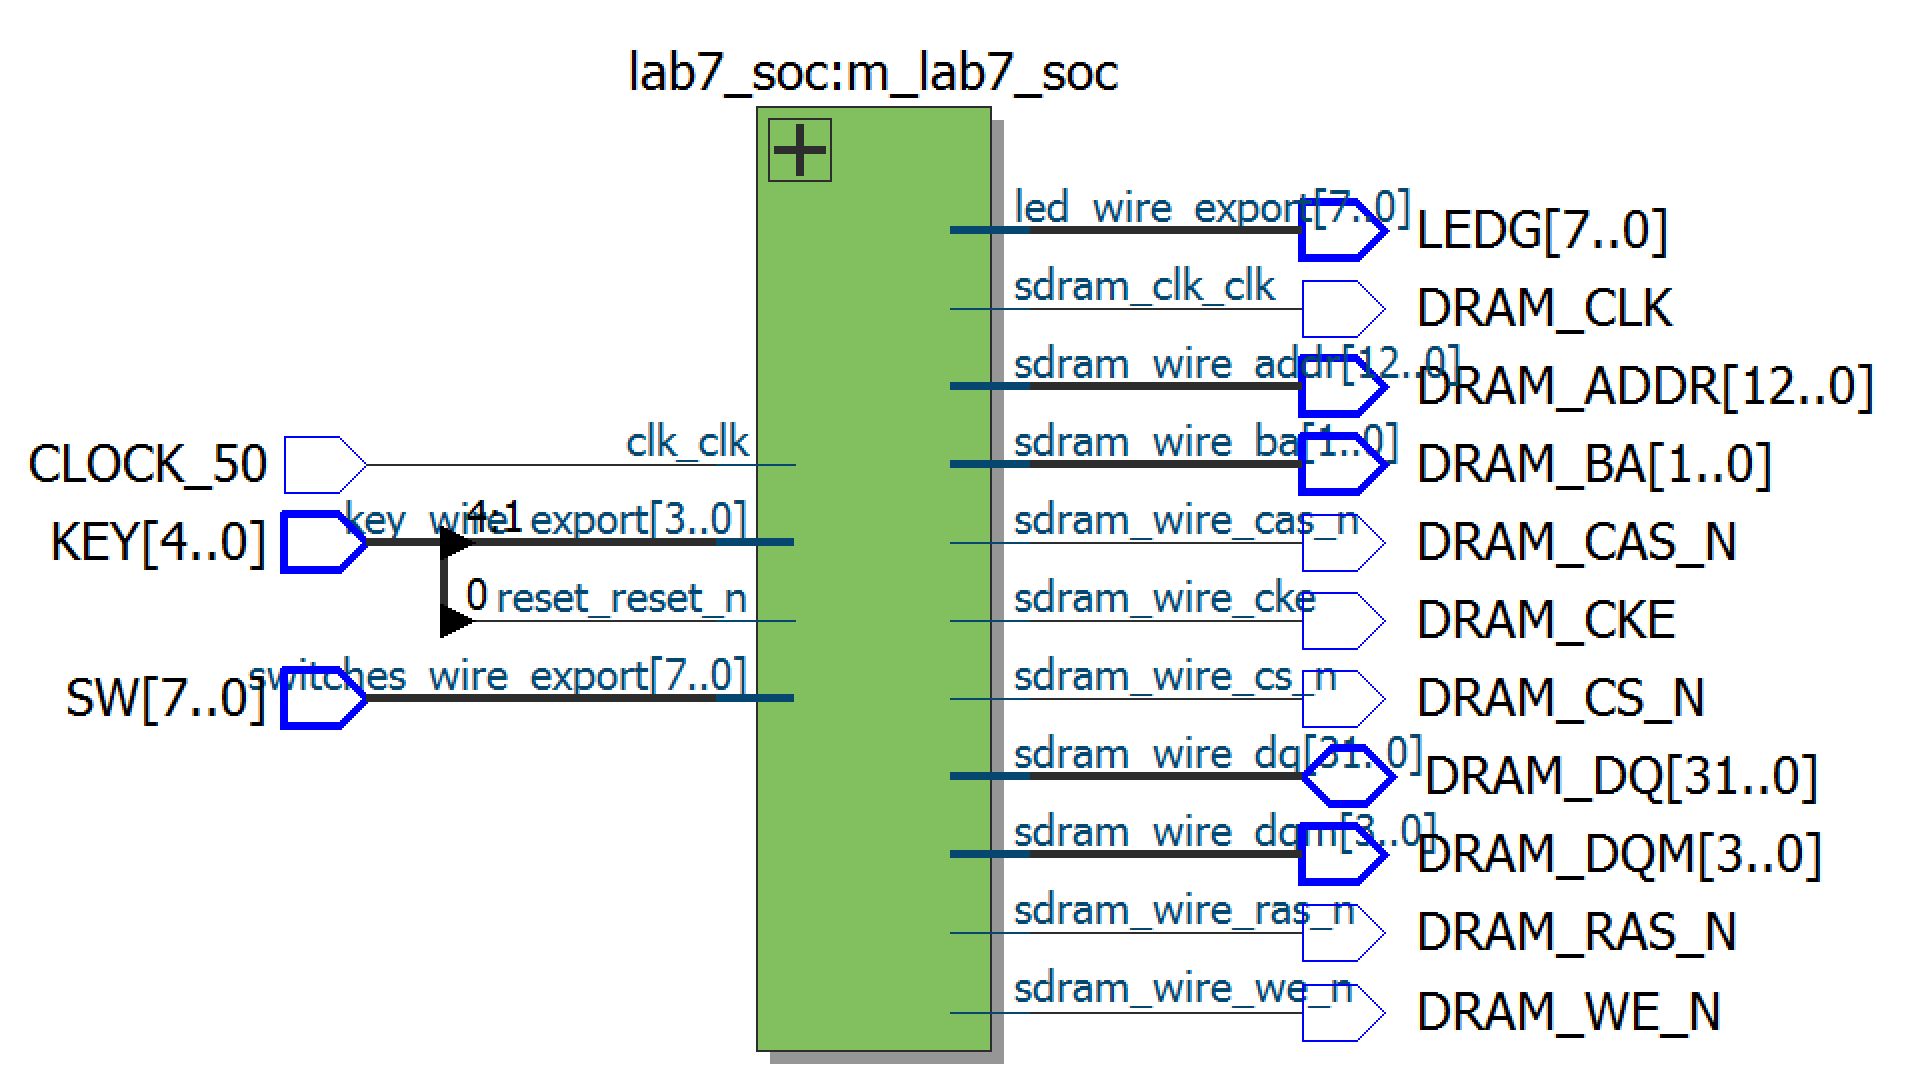
\includegraphics[scale=0.4]{top-top-circuit.png}
	\caption{Lab7 Top Level Block Schematic\label{fig:top-level}}
\end{figure}

\begin{figure} [H]
	\centering
	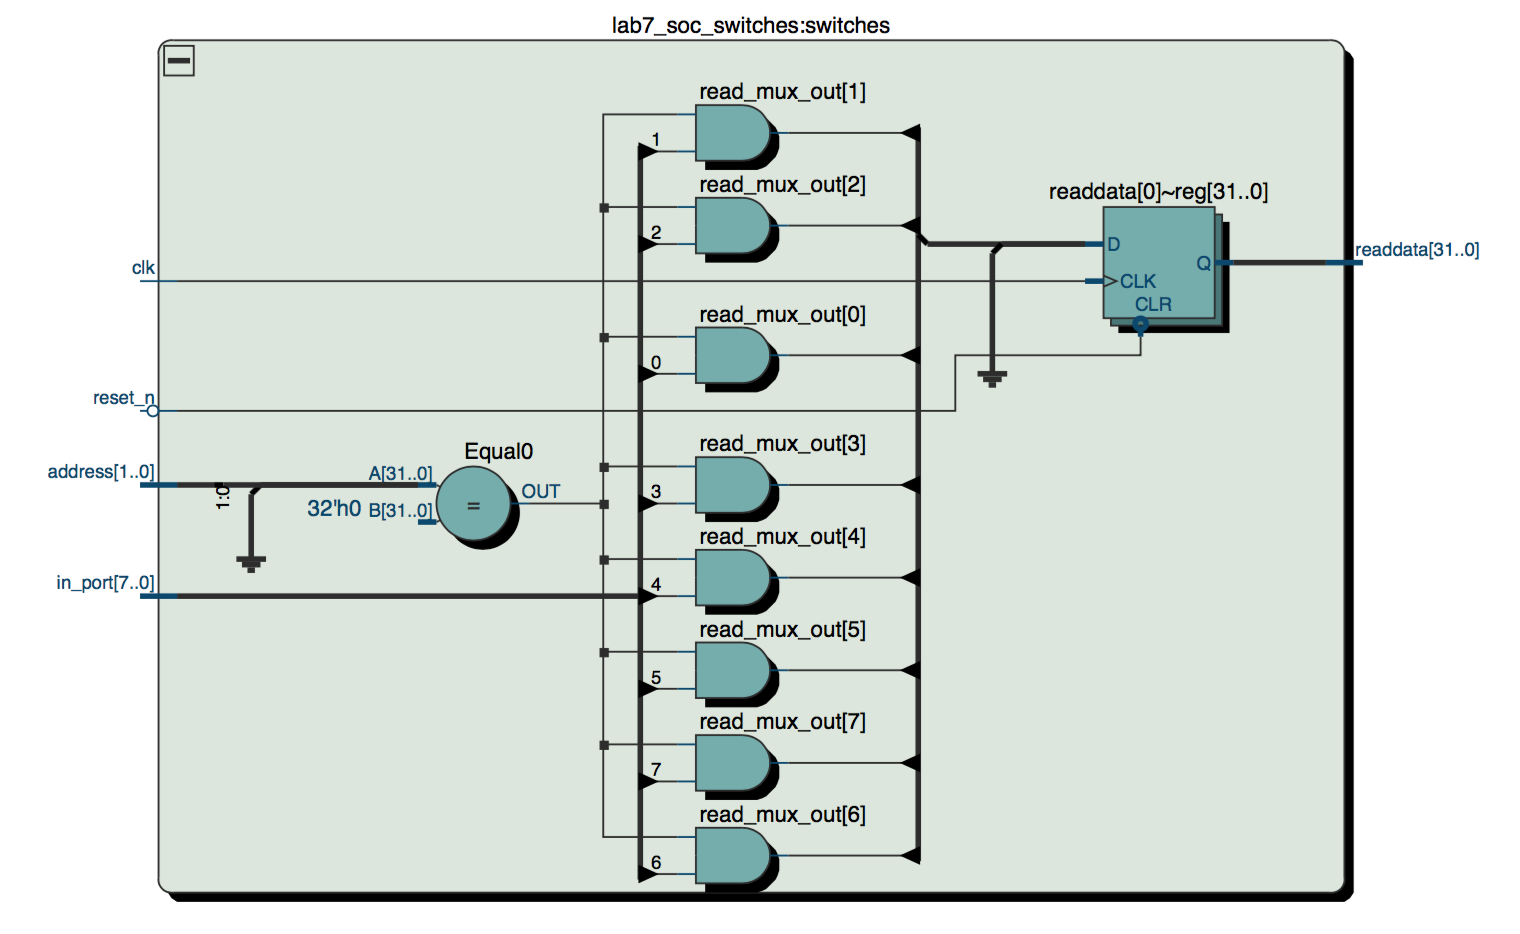
\includegraphics[scale=0.4]{switches_pio_module.png}
	\caption{Switches PIO Module\label{fig:switch-pio}}
\end{figure}

\begin{figure} [H]
	\centering
	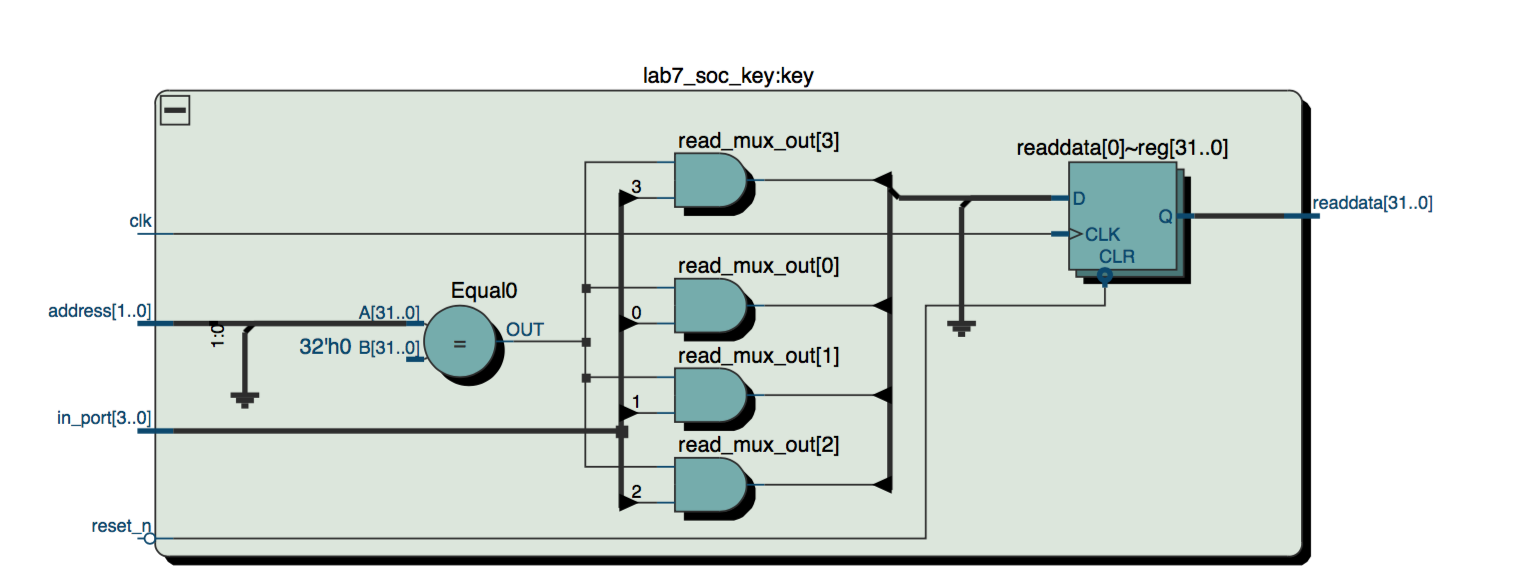
\includegraphics[scale=0.4]{key_pio_module.png}
	\caption{Key PIO Module\label{fig:key-pio}}
\end{figure}

\begin{figure} [H]
	\centering
	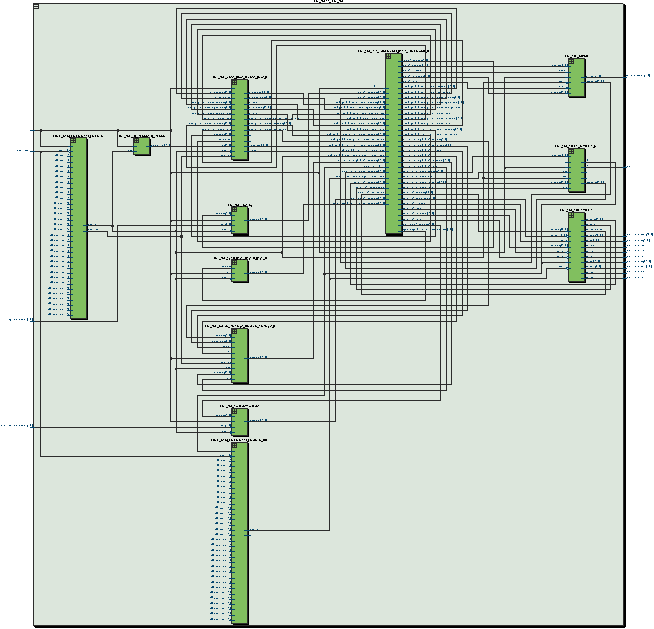
\includegraphics[scale=1.72]{top-level-circuit.pdf}
	\caption{Lab 7 Module Interconnections\label{fig:top-level-interconn}}
\end{figure}


%SECTION : Bibliography
%Insert Bibliography if needed

\end{document}
